\documentclass[11pt]{article}
% \pagestyle{empty}

\setlength{\oddsidemargin}{-0.25 in}
\setlength{\evensidemargin}{-0.25 in}
\setlength{\topmargin}{-0.9 in}
\setlength{\textwidth}{7.0 in}
\setlength{\textheight}{9.0 in}
\setlength{\headsep}{0.75 in}
\setlength{\parindent}{0.3 in}
\setlength{\parskip}{0.1 in}
\usepackage{epsf}
\usepackage{pseudocode}
\usepackage{ amssymb }
\usepackage{tikz}
\usepackage{listings}
\usetikzlibrary{arrows.meta}
\usepackage{algorithmic}
\usepackage{changepage}
\usepackage{lipsum}
\usepackage{enumitem}
\usepackage{indentfirst}
\usepackage{amsmath}
\usepackage{graphicx}
\graphicspath{ {desktop/} }


% \usepackage{times}
% \usepackage{mathptm}

\def\O{\mathop{\smash{O}}\nolimits}
\def\o{\mathop{\smash{o}}\nolimits}
\newcommand{\e}{{\rm e}}
\newcommand{\R}{{\bf R}}
\newcommand{\Z}{{\bf Z}}
\newcommand{\findent}{\leavevmode{\parindent=2em\indent}}
\newcommand\solution{%
  \textbf{Solution.}\\%
}
\begin{document}

CS 124 Problem Set 5 \\
\indent HARVARD ID: 10939860

\begin{enumerate}

\item

\solution \\
First, consider the probability that no two people receive the same hash value, which (similar to the birthday problem) can be represented as: 
\begin{equation*}
  \prod_{i=1}^{c_i \sqrt{n} - 1} (1-\frac{i}{n})
\end{equation*}
From the hint, we can conclude that 
\begin{equation*}
  \prod_{i=1}^{c_i \sqrt{n} - 1} (1-\frac{i}{n}) < \prod_{i=1}^{c_i \sqrt{n} - 1} e^{-\frac{i}{n}}
\end{equation*}
so we will find a constant $c_1$ to show that the probability that no two people have the same hash is at most $\frac{1}{e}$ when there are at least $c_1 \sqrt{n}$ in the room:
\begin{equation*}
  e^{\sum_{i=1}^{c_1 \sqrt{n} - 1} -\frac{i}{n}} = e^{\frac{-(c_1 \sqrt{n})(c_1 \sqrt{n})}{2n}} = e^{\frac{-c_1^2 n + c_1 \sqrt{n}}{2n}}
\end{equation*}
From here, set the equation to be less than or equal to $\frac{1}{e}$ and use algebra:
\begin{equation*}
  e^{\frac{-c_1^2 n + c_1 \sqrt{n}}{2n}} \leq \frac{1}{e}
\end{equation*}
\begin{equation*}
  \frac{-c_1^2}{2} + \frac{c_1 \sqrt{n}}{2n} \leq -1
\end{equation*}
\begin{equation*}
  \frac{c_1^2}{2} + \frac{c_1}{2\sqrt{n}} \geq 1
\end{equation*}
Next, take the limit as $n$ goes to infinity, to get rid of the $n$ value and consider $c_1$ for sufficiently large $n$:
\begin{equation*}
  \displaystyle \lim_{n \to \infty} (\frac{c_1^2}{2} + \frac{c_1}{2\sqrt{n}})
\end{equation*}
\begin{equation*}
  \frac{c_1^2}{2} \geq 1
\end{equation*}
\begin{equation*}
  c_1 \geq \sqrt{2}
\end{equation*}
Thus, we can conclude that there exists a constant $c_1$ that satisfies the probability inequality given in the problem. \\
\\
For the second part of the question, we use similar logic, beginning with the same product for the probability, instead setting it greater or equal than $\frac{1}{2}$, since we aim to prove that the probability that no two have the same hash is at least $\frac{1}{2}$ when there are at most $c_2 \sqrt{n}$ people in the room for some $c_2$. We begin from a point in part 1 of the problem where we had simplified this probability:
\begin{equation*}
  \prod_{i=1}^{c_2 \sqrt{n} - 1} e^{-\frac{i}{n}} = e^{\frac{-c_2^2 n + c_2 \sqrt{n}}{2n}}
\end{equation*}
\begin{equation*}
  e^{\frac{-c_2^2 n + c_2 \sqrt{n}}{2n}} \geq \frac{1}{2}
\end{equation*}
Using algebra, 
\begin{equation*}
  -\frac{c_2^2}{2} + \frac{c_2}{2\sqrt{n}} \geq ln(\frac{1}{2})
\end{equation*}
\begin{equation*}
  -\frac{c_2^2}{2} + \frac{c_2}{2\sqrt{n}} \geq ln(1) - ln(2)
\end{equation*}
\begin{equation*}
  \frac{c_2^2}{2} - \frac{c_2}{2\sqrt{n}} \leq ln(2)
\end{equation*}
As in part 1, we take the limit as $n$ approaches infinity to simplify the equation to solve for $c_2$ and account for sufficiently large $n$: 
\begin{equation*}
  \displaystyle \lim_{n \to \infty} \frac{c_2^2}{2} - \frac{c_2}{2\sqrt{n}} = \frac{c_2^2}{2} \leq ln(2)
\end{equation*}
\begin{equation*}
  c_2 \leq \sqrt{2ln(2)}
\end{equation*}
Thus, we have shown that for $c_2$ under this constraint, the probability that no two have the same hash is at least $\frac{1}{2}$ when there are at most $c_2 \sqrt{n}$ people in the room.

\item

\solution \\
To consider the probability that a specific counter will overflow in this modified bloom filter model, we can use the binomial distribution, viewing hashing into the same specific location as a "success" and hashing into any other location as a "failure." For a 3-bit counter, a specific counter will overflow after 8 hashes in a specific location. Stemming from the binomial formula, letting A be the event of at least 8 successes, we see that 
\begin{equation*}
  P(A) = 1 - \sum_{i = 0}^{7} {n \choose i} (\frac{k}{m})^i (1-\frac{k}{m})^{n-i} = 1 - \sum_{i = 0}^{7} {10^5 \choose i} (\frac{10ln(2)}{10^6})^i (1-\frac{10ln(2)}{10^6})^{n-i} = 7.15 x 10^{-8}
\end{equation*}
This makes sense, as any hash has probability $k/m$ of landing in a particular location, so we must take that into account as well as the probability of landing in any other spot, choosing which location to consider and summing over the possibility of 0 to 7 successes. Finally, we take the complement to find the probability of at least 8 successes, or hashes in a particular location. \\
\\
For a 4-bit counter, we will have the same equation, though with a different summation, as any specific counter will take 16 hashes in that location to overflow the counter, so we sum over 0 to 15 successes and take the complement, letting B be the event of at least 16 successes:
\begin{equation*}
  P(B) = 1 - \sum_{i = 0}^{15} {n \choose i} (\frac{k}{m})^i (1-\frac{k}{m})^{n-i} = 7.07 x 10^{-17}
\end{equation*}
Continuing, the pattern remains for a 5-bit counter, but with 32 hashes in a single location. We sum over 0 to 31 successes and take the complement, letting C be the event of at least 32 successes:
\begin{equation*}
  P(C) = 1 - \sum_{i = 0}^{7} {n \choose i} (\frac{k}{m})^i (1-\frac{k}{m})^{n-i} = 1.56 x 10^{-41}
\end{equation*}
In practice, a 4-bit counter seems smart to use. We must consider the space and efficiency tradeoff. While the 4-bit counter implementation will take more space than the 3-bit, the 3-bit probability, while very small, could result in overflow for large data sets. The 4-bit counter implementation probability is small enough to feel comfortable on large data sets.

\item 

\solution \\
Similar to problem 2, we can think of this probability as a binomial formula. Essentially, we have a balls and bins problem with 6 balls and $2^{64}$ bins. If we define a success to be two sketches matching to the same bucket out of the $2^{64}$ sketches, the probability that two documents with resemblance $r$ agree on two or more of the six sketches can be directly translated to the binomial distribution. The probability of an individual success is $r^{14}$ because there are 14 values within each sketch that need to be matched. Letting A be the event that at least two of the six sketches match, we have 
\begin{equation*}
  P(A) = \sum_{i = 2}^{6} {6 \choose i} (r^{14})^i (1-r^{14})^{6-i}
\end{equation*}
since we must sum over the probabilities that 2, 3, 4, 5, or 6 of the sketches match. \\
\\
We can assume that it makes sense that this is the only time that a match will occur, because the probability of a false positive is extremely small: for a 64-bit hash, the probability of a sketch landing in the same bin even if it shouldn't is $\frac{1}{2^{64}}$. This is close enough to 0 that the probability is negligible. However, for a 16-bit hash, the probability is $\frac{1}{2^{16}} = \frac{1}{65536}$, and for an 8-bit hash, the probability of a false positive is even more likely at $\frac{1}{2^8} = \frac{1}{256}$. For many trials, both of these probabilities make it fairly likely for false positives to occur, so we can't assume that the sketches indicate a correct match in all cases. Thus, in practice, using a 64-bit hash is much more accurate. \\
\\
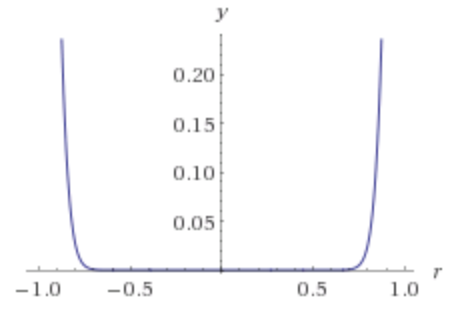
\includegraphics{ps5graph} \\
See the above graph for a graph of the probability. It looks very similar to the document similarity problem graph in class, which makes sense. When the resemblance is very low, the probability of at least two sketches matching is near 0, but as the resemblance shoots up, the probability rises quickly along with it. 

\item 

\solution \\
We will modify the fingerprinting algorithm discussed in class. First, create a new hash table, using just one hash function. Use this hash function to hash each of the $k$ patterns, returning a number for each. Initialize the resulting hashes as the keys in the aforementioned hash table, with the value as an index for each hash. For example, letting the patterns be labeled $p_1, p_2, .., p_k$, let our hash table map $hash(p_1)$ to $1$, ...,  $hash(p_k)$ to $k$. \\
\\
Next, look at each pattern of size $|P|$ in the document, reading through just once. At each step, hash the corresponding pattern of size $|P|$, checking if the resulting hash is a key in the hash table (achieved in constant lookup time). If the hash is in the hash table, then return the value mapped to by that key, giving the pattern number associated with the pattern in the document. Otherwise, simply continue to the next pattern in the document until the end. \\
\\
This modified algorithm will affect the probability of false positives by a factor of $k$ at every step. The expectation stays the same, but the new probability of a false positive is:
\begin{equation*}
  \frac{k*|D| log_2 10^{|P|}}{\pi(z)}
\end{equation*}
The algorithm is better than the original fingerprinting method, as it runs in more efficient time and takes the same amount of space. 

\item 

\solution \\
The relevant code for this question is attached as $ps5\_composite.py$. In it, I simply implement a form of the Rabin-Miller algorithm. First, there is a helper function for exponentiation by squaring, and then a Rabin-Miller test to take in an $n$ and $a$. I hard-code in values for $a$ to find the lowest witness to prove that $n$ is composite. The function returns "PRIME" if $is\_composite = False$ and "COMPOSITE" if $is\_composite = True$. \\
\\
The logic of the code is easy to follow, directly following the process of Rabin-Miller that we learned in class. At various points, it changes the boolean value to indicate if $n$ is composite or not. I tested the numbers 294409 and 636127 with multiple witnesses, and saw that $a = 2$ served as a witness for proving that both numbers are composite. I also tested nearby prime numbers to make sure that the algorithm returned "PRIME" for all values of $a$. Thus, I know that the witness is in fact a witness due to the implementation of Rabin-Miller. \\
\\
Fermat's little theorem will not work for the 294409 case because the theorem is an if, not an if and only if, meaning it is only one way. For Carmichael numbers, a number may be n-pseudoprime, passing the primality test of Fermat's little theorem even if it is not actually prime. 

\item 

\solution \\
The relevant code is attached as $ps5\_rsa.py$. This is a straightforward implementation of the RSA cryptography algorithm with a given public key. I implemented a exponentiation by squaring helper function that also mods by a number at every step (basically re-implementing the Python system pow function). I then enter the string and public key, translating the string to binary and performing the algorithm's calculations. Running this script, I calculated the encoded message in decimal as 27016764340118192395712492378. 

\item 

\solution \\
The relevant code is attached as $ps5\_ballsbins.java$. The code is not completely correct and I acknowledge that, but I didn't have time to completely finish it. Running the code a few times, I computed the maximum load as various values of 1,2, and 3 that didn't seem correct to me. However, I will discuss my logic in the code. \\
\\
For this algorithm, I initialize an array, $B$, which begins with $B[0] = 1000000000$. The array is set up so that $B[i] = n$ where $n$ bins have $i$ balls. We run a for loop 100000000 times, where $B[0]$ decrements with each iterations as other indices incrementing their counter (i.e. $B[1]$ incrementing very often). We order the bins, choose a random number between 1 and 1000000000, initialize an array of size 50 (arbitrary) to represent the array of size 1000000000, and then test if the random number is less than or equal to $B[i]$. If it is, then decrement $B[0]$ by 1 and increment $B[1]$ by 1. If not, then increment some counter to find the proper indices to increment and decrement until we get the case that the random number is less than $B[i]$. \\
\\
For the second part of the question, modify the algorithm to generate two random numbers instead of one, choosing the minimum of the two to perform the exact same algorithm described above. This will ensure that we put the ball in the least loaded of the two bins. Generally, this algorithm is much more efficient in time and space than keeping an array of 1000000000 bins. 



\end{enumerate}
\end{document}
